%% Report on tau -> mu gamma and tau -> e gamma in the S3-3HDM: exact and soft-broken vacua.
%% Companion: derivations_08.tex (the derivation ledger, auto-generated by the notebook).
%% Source: research/thdm_s3/08_tau_to_l_gamma.ipynb
\documentclass[11pt,a4paper]{article}
\usepackage[T1]{fontenc}
\usepackage[utf8]{inputenc}
\usepackage{amsmath,amssymb}
\usepackage{graphicx}
\usepackage{booktabs}
\usepackage[margin=2.4cm]{geometry}
\usepackage[colorlinks=true,linkcolor=blue,citecolor=blue,urlcolor=blue]{hyperref}
% Generated by report_numbers.py from results/*.json -- do not edit by hand.
% Use as \macro{} in text; the sample sizes belong in maths mode.
\newcommand{\nExactPoints}{1973}  % points surviving the exact-S3 scan (viable_points.json: n_points)
\newcommand{\nExactSample}{6\times10^{7}}  % points sampled in the exact-S3 scan (use in maths mode) (viable_points.json: sample_size)
\newcommand{\nSoftPoints}{2028}  % points surviving the soft-broken scan (viable_points_soft.json: n_points)
\newcommand{\nSoftSample}{1.1\times10^{8}}  % points sampled in the soft-broken scan (use in maths mode) (viable_points_soft.json: sample_size)
\newcommand{\nLFVexcluded}{5}  % soft points with no lepton configuration under the h->ll' limits (soft_decay_benchmarks.json: n_points_lfv_excluded_for_every_lepton_config)
\newcommand{\nMuEConfigs}{417\,992}  % (point, mu3, branch) configurations in the soft scan (mu_e_gamma.json: summary/n_configurations)
\newcommand{\fMEGconfigs}{2.51\%}  % fraction of configurations under MEG II (mu_e_gamma.json: summary/frac_configurations_under_meg)
\newcommand{\nHLFVallowed}{2023}  % soft points allowed by the h->ll' limits (mu_e_gamma.json: summary/n_points_allowed_h)
\newcommand{\nMEGallowed}{618}  % soft points allowed by MEG II (mu_e_gamma.json: summary/n_points_allowed_meg)
\newcommand{\nBothAllowed}{606}  % soft points allowed by MEG II and the h->ll' limits (mu_e_gamma.json: summary/n_points_allowed_both)
\newcommand{\nMEGnoQuark}{504}  % MEG II survivors without the quark Barr-Zee term (mu_e_gamma.json: summary/n_points_allowed_meg_variants/no_quark)
\newcommand{\nMEGtopFlip}{453}  % MEG II survivors with the quark couplings' sign flipped (mu_e_gamma.json: summary/n_points_allowed_meg_variants/top_flip)
\newcommand{\nMEGwHKZ}{684}  % MEG II survivors with the W loop at the HKZ13 value (mu_e_gamma.json: summary/n_points_allowed_meg_variants/w_hkz)
\newcommand{\xMEGmedianBR}{7.6\times10^{-10}}  % median B(mu -> e gamma) over the configurations (use in maths mode) (mu_e_gamma.json: summary/median_br)
\newcommand{\xMEGoverHemu}{9.1\times10^{4}}  % median (B/MEG)/(B(h->e mu)/CMS) per configuration (use in maths mode) (mu_e_gamma.json: summary/median_meg_over_hemu_ratio)
\newcommand{\nTauConfigs}{417\,992}  % (point, mu3, branch) configurations in the tau scan (tau_l_gamma.json: summary/n_configurations)
\newcommand{\nExactEvals}{118\,380}  % (exact point, mu3) evaluations at the exact-S3 vacuum (tau_l_gamma.json: summary/exact/n_evaluations)
\newcommand{\fExactOverBelle}{0.72\%}  % exact-vacuum evaluations over the Belle tau->mu gamma limit (tau_l_gamma.json: summary/exact/frac_over_belle)
\newcommand{\fExactOverCMS}{18.5\%}  % exact-vacuum evaluations over the CMS h->tau mu limit (tau_l_gamma.json: summary/exact/frac_over_cms_taumu)
\newcommand{\nExactBelleNotCMS}{460}  % exact-vacuum evaluations over Belle but under CMS h->tau mu (tau_l_gamma.json: summary/exact/n_over_belle_under_cms)
\newcommand{\fSoftOverBelle}{0.020\%}  % soft configurations over the Belle tau->mu gamma limit (tau_l_gamma.json: summary/frac_configurations_over_limit/tau_mu)
\newcommand{\fSoftOverBaBar}{0.029\%}  % soft configurations over the BaBar tau->e gamma limit (tau_l_gamma.json: summary/frac_configurations_over_limit/tau_e)
\newcommand{\nTauBothAllowed}{2028}  % soft points with a configuration under both tau limits (tau_l_gamma.json: summary/n_points_allowed/tau_both)
\newcommand{\nAllRadAllowed}{618}  % soft points under all three radiative limits (tau_l_gamma.json: summary/n_points_allowed/all_rad)
\newcommand{\nAllRadHAllowed}{606}  % soft points under all three radiative and the h->ll' limits (tau_l_gamma.json: summary/n_points_allowed/all_rad_h)
\newcommand{\nRadNoQuark}{504}  % all-radiative survivors without the quark Barr-Zee term (tau_l_gamma.json: summary/n_points_allowed_all_radiative_variants/no_quark)
\newcommand{\nRadTopFlip}{453}  % all-radiative survivors with the quark couplings' sign flipped (tau_l_gamma.json: summary/n_points_allowed_all_radiative_variants/top_flip)
\newcommand{\nRadwHKZ}{684}  % all-radiative survivors with the W loop at the HKZ13 value (tau_l_gamma.json: summary/n_points_allowed_all_radiative_variants/w_hkz)
  % headline numbers, generated by report_numbers.py
\setlength{\parindent}{0pt}
\setlength{\parskip}{0.6em}

\title{$\tau\to\mu\gamma$ and $\tau\to e\gamma$ in the $S_3$ 3HDM:\\
allowed at the exact vacuum,\\
and no new constraint in the soft one}
\author{M. Zeleny-Mora\\[2pt]
\small Instituto de Física, Universidad Nacional Autónoma de México}
\date{\today}

\begin{document}
\maketitle

\begin{abstract}
\noindent
This report completes the three radiative LFV decays $\ell_i\to\ell_j\gamma$ on the same
\nSoftPoints{} soft-broken points as the $\mu\to e\gamma$ report, and adds the
\nExactPoints{} exact-$S_3$ points, which $\mu\to e\gamma$ cannot test. The diagrams are the
same; only the flavour indices and the $\tau$ normalization change, and both are checked
against independent sources. At the exact vacuum the residual $\mathbb Z_2$ splits the two
channels: $\tau\to e\gamma$ vanishes identically, while $\tau\to\mu\gamma$ is allowed and
generic. The Belle limit \cite{Belle21} excludes only \fExactOverBelle{} of the exact
configurations, far fewer than $h\to\tau\mu$, but \emph{not a subset} of them: where a non-SM
$\mathbb Z_2$-even scalar is light, $\tau\to\mu\gamma$ excludes what the Higgs decay allows.
In the soft vacuum the $\tau$ modes add nothing beyond MEG~II: every scalar point keeps a
$\tau$-allowed configuration, and the counts stay at \textbf{\nAllRadAllowed{} of
\nSoftPoints{}} (\nAllRadHAllowed{} with the Higgs LFV limits). Where every limit holds the
$\tau$ rates stay below $5\times10^{-10}$, an order of magnitude under the projected reach of
Belle~II.
\end{abstract}

\section{Summary}

Everything below comes from \texttt{research/thdm\_s3/08\_tau\_to\_l\_gamma.ipynb}, with the
numerics in \texttt{radiative.py} and \texttt{soft\_decays.py}; the two scans run in
\texttt{compute\_tau\_l\_gamma.py}.

\begin{enumerate}\itemsep2pt
\item \textbf{The generalization to $\ell_i\to\ell_j\gamma$ is checked}, not assumed
(\S\ref{sec:general}).
\item \textbf{For an SM-like Higgs the Higgs decay wins in the $\tau$ sector}, by about
$12\times$ in the coupling: the reverse of the $e\mu$ sector (\S\ref{sec:sm}).
\item \textbf{Exact $S_3$: $\tau\to e\gamma=0$, $\tau\to\mu\gamma\neq0$}, and Belle removes a
light-scalar corner that $h\to\tau\mu$ misses (\S\ref{sec:exact}).
\item \textbf{Soft vacuum: no point removed beyond MEG~II} (\S\ref{sec:scan}).
\item \textbf{A prediction for Belle~II} (\S\ref{sec:belle2}).
\end{enumerate}

\section{From $\mu\to e\gamma$ to $\ell_i\to\ell_j\gamma$}
\label{sec:general}

The amplitude of the previous report carries over with the decaying lepton $i$ and the final
one $j$ as arguments. The neutral one loop becomes
\[
c_L=\sum_{f}\frac{\tfrac12I_1(t_f)\,(m_jY_{jf}Y^*_{if}+m_iY^*_{fj}Y_{fi})
+I_2(t_f)\,m_fY^*_{fj}Y^*_{if}}{4m_im_\phi^2},\qquad A=\frac{c}{4\pi^2},
\]
the charged loop is $A_L=-(Y_C^\dagger Y_C)_{ji}/(192\pi^2m_{H^\pm}^2)$, and the Barr--Zee
terms take $(Y_{ij},Y_{ji})$ and $1/m_i$ in place of $(Y_{\mu e},Y_{e\mu})$ and $1/m_\mu$.
Two things are new physics rather than plumbing:
\begin{itemize}\itemsep0pt
\item the internal-$\tau$ chirality flip, which dominates the one loop of $\mu\to e\gamma$
($\propto m_\tau/m_\mu$), is \textbf{not enhanced} for a decaying $\tau$ ($m_\tau/m_\tau$,
times a logarithm);
\item the width is normalized to $\Gamma(\tau\to\ell\nu\bar\nu)$ and multiplied by its
branching ratio \cite{OST16}, Eq.~(17):
\[
\mathcal B(\tau\to\ell\gamma)=\frac{48\pi^3\alpha\,(|A_L|^2+|A_R|^2)}{G_F^2}\,
\mathcal B(\tau\to\ell\nu\bar\nu).
\]
\end{itemize}

\begin{center}
\begin{tabular}{lll}
\toprule
check & against & agreement\\
\midrule
$(i,j)=(\mu,e)$, 25 points & stored $\mu\to e\gamma$ results (4 figures) & $3.5\times10^{-4}$\\
relabelling $(e,\mu,\tau)\to(\mu,\tau,e)$ & the $(\mu,e)$ code & $3\times10^{-16}$\\
closed-form one loop, $\tau\to\mu\gamma$ & \cite{HKZ13} (A3), external masses kept & $3\times10^{-6}$ / $2\times10^{-3}$ (700 / 25~GeV)\\
one loop, internal $\tau$ only & \cite{OST16} Eq.~(19) & $10^{-4}$\\
$\tau$ normalization & \cite{HKZ13}'s lifetime normalization, \cite{PDG} & 0.2\%\\
$\tau\to\mu\gamma$, $\tau\to e\gamma$ bounds & \cite{HKZ13}: 0.016, 0.014 & 0.0159, 0.0136\\
\bottomrule
\end{tabular}
\end{center}

The relabelling test uses the couplings of a real soft point and shows that no fixed $e$ or
$\mu$ index survived in the general code. The \cite{OST16} Eq.~(19) check also confirms where
$m_i$ and $m_f$ sit: the flip and non-flip terms there carry the same mass, and a version with
the $m_\tau/m_\mu$ flip factor of $\mu\to e\gamma$ carried over fails it. The \cite{HKZ13}
bounds are reproduced with their $W$-loop number (the previous report found ours 14\% above
it). In the $\tau$ channels the one loop is comparable to the two loop, so this oracle also
fixes their relative sign; flipping it fails the comparison.

\section{An SM-like Higgs: the Higgs decay is stronger here}
\label{sec:sm}

At the current limits and pole $m_t$, an SM-like Higgs needs
\[
\sqrt{|Y_{\tau\mu}|^2+|Y_{\mu\tau}|^2}<0.013\ \text{(Belle)},\qquad
\sqrt{|Y_{\tau e}|^2+|Y_{e\tau}|^2}<0.011\ \text{(BaBar)},
\]
while the CMS searches for $h\to\tau\mu$ and $h\to\tau e$ \cite{CMS21} need 0.0011 and 0.0013.
In the $\tau$ sector \textbf{the Higgs decay is $12\times$ and $8\times$ stronger in the
coupling}. This is the reverse of the $e\mu$ case, where MEG~II bounds the coupling at
$7\times10^{-7}$ against $10^{-4}$ for $h\to e\mu$. The $\tau$ modes can still matter where
the Higgs decay is blind: the LFV couplings of the \emph{non-SM} scalars.

\section{The exact-$S_3$ vacuum: $\tau\to e\gamma$ vanishes, $\tau\to\mu\gamma$ does not}
\label{sec:exact}

The previous report traced the zero of $\mu\to e\gamma$ at the exact vacuum to its residual
$\mathbb Z_2$. Under it the electron and the in-plane non-vacuum scalars ($h_0$, one $A$, one
$H^\pm$) are odd, and $\mu$, $\tau$ even. So $\tau\to e\gamma$, with one odd lepton, is
forbidden, while $\tau\to\mu\gamma$, with none, is allowed through the even scalars. The
exact points, which $\mu\to e\gamma$ cannot test, meet their first radiative constraint here.

Each of the \nExactPoints{} exact points is evaluated at $\varphi=\pi/3$ with every free soft
term zero, on the draft lepton branch, at 60 values of $\mu_3\in(m_\mu,m_\tau)$: \nExactEvals{}
evaluations.

\begin{itemize}\itemsep2pt
\item $\mathcal B(\tau\to e\gamma)<10^{-33}$ and $\mathcal B(\mu\to e\gamma)<10^{-29}$
everywhere, which is round-off, although single $e\tau$ couplings reach 0.09.
\item Every evaluation shows the pattern behind it: three odd states with no $\tau\mu$
coupling, and four even states with no coupling to the electron.
\item Off the alignment, with one exact point and the free soft terms still zero,
$\mathcal B(\tau\to e\gamma)\propto(60^\circ-\varphi)^2$ (fitted slope 2.00), as for
$\mu\to e\gamma$.
\item $\tau\to\mu\gamma$ is generic: median $2.1\times10^{-11}$, maximum $1.1\times10^{-4}$.
\end{itemize}

\begin{center}
\begin{tabular}{lc}
\toprule
& exact-vacuum evaluations excluded\\
\midrule
Belle, $\tau\to\mu\gamma$ \cite{Belle21} & \fExactOverBelle{}\\
CMS, $h_{\rm SM}\to\tau\mu$ \cite{CMS21} & \fExactOverCMS{}\\
Belle but not CMS & \nExactBelleNotCMS{} evaluations, at 20 points\\
\bottomrule
\end{tabular}
\end{center}

\textbf{The light-scalar corner.} The Belle exclusion is thin but not contained in the CMS
one. In all \nExactBelleNotCMS{} evaluations that only Belle excludes, the one loop is the
largest piece, and a non-SM neutral $\mathbb Z_2$-even scalar is light: 6.7--223~GeV, against
a median of 302~GeV over all exact points. Its $\tau\mu$ coupling enters with
$1/m_\phi^2$, and the SM-like Higgs decay cannot see that state. The closed-form one loop
still holds there, to $1.3\times10^{-2}$ at 6.7~GeV against the full \cite{HKZ13} integral.
No exact point loses its whole $\mu_3$ range.

\textbf{The $S_3$ image.} $\varphi\to2\pi/3-\varphi$, with both soft doublets reflected, is
the same physics: all three branching ratios agree at a point and at its image to
$4\times10^{-10}$ (20 points, every configuration).

\section{The soft-broken scan}
\label{sec:scan}

Every point $\times$ the 73-value $\mu_3$ grid $\times$ every lepton branch gives
\nTauConfigs{} configurations, with all three channels and the SM-like state's
$h\to\ell\ell'$ rates computed together. The medians are
$\mathcal B(\tau\to\mu\gamma)=2.2\times10^{-12}$ and $\mathcal B(\tau\to e\gamma)=2.3\times10^{-12}$,
and only \fSoftOverBelle{} and \fSoftOverBaBar{} of the configurations exceed Belle and
BaBar \cite{BaBar10}.

\begin{center}
\begin{tabular}{lc}
\toprule
limits applied & scalar points with an allowed configuration\\
\midrule
$\tau\to\mu\gamma$ and $\tau\to e\gamma$ & \nTauBothAllowed{} / \nSoftPoints{}\\
MEG~II \cite{MEGII25} & \nMEGallowed{} / \nSoftPoints{}\\
all three radiative & \textbf{\nAllRadAllowed{} / \nSoftPoints{}}\\
all three radiative and the $h\to\ell\ell'$ limits \cite{CMS21,CMS23} & \nAllRadHAllowed{} / \nSoftPoints{}\\
\bottomrule
\end{tabular}
\end{center}

Adding both $\tau$ limits to MEG~II removes no point. Configuration by configuration, measured
against its own limit, $\tau\to\mu\gamma$ is a median $9\times10^{-3}$ as restrictive as
$h\to\tau\mu$, and only 108 configurations are excluded by a $\tau$ mode while allowed by every
Higgs LFV limit. The $W$-loop Barr--Zee diagram is the largest piece of both $\tau$ channels in
93\% of configurations, as for $\mu\to e\gamma$.

\begin{figure}[h]
\centering
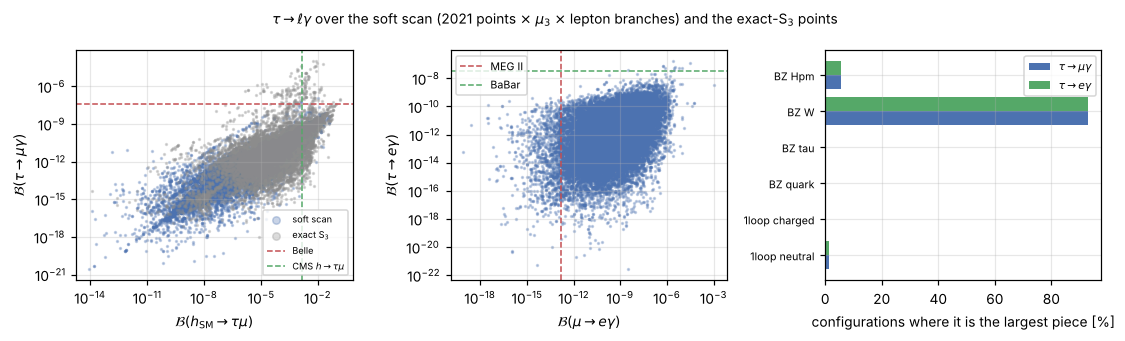
\includegraphics[width=\textwidth]{figures/tau_l_gamma_scan.png}
\caption{Left: $\mathcal B(\tau\to\mu\gamma)$ against the SM-like $\mathcal B(h\to\tau\mu)$
per configuration, soft scan (blue, 40\,000 sampled) and exact-$S_3$ points (grey), with the
Belle and CMS limits dashed. Middle: $\mathcal B(\tau\to e\gamma)$ against
$\mathcal B(\mu\to e\gamma)$ in the soft scan, with the BaBar and MEG~II limits. Right: which
piece of the amplitude is largest, by share of configurations.}
\label{fig:scan}
\end{figure}

\textbf{Robustness.} The same three variants as in the $\mu\to e\gamma$ report, built from
the same amplitudes for every channel:

\begin{center}
\begin{tabular}{lc}
\toprule
variant & scalar points allowed by all three radiative limits\\
\midrule
baseline & \nAllRadAllowed{}\\
no quark Barr--Zee & \nRadNoQuark{}\\
quark couplings with opposite sign & \nRadTopFlip{}\\
$W$ loop scaled to \cite{HKZ13}'s 0.11 & \nRadwHKZ{}\\
\bottomrule
\end{tabular}
\end{center}

In each variant the counts equal the MEG~II-only ones of the previous report: the $\tau$ modes
remove no point under any of them.

\section{A prediction for Belle~II}
\label{sec:belle2}

$\mathcal B(\tau\to e\gamma)/\mathcal B(\mu\to e\gamma)$ has median $2.8\times10^{-3}$. In the
MEG-allowed configurations the $\tau$ rates stay at or below $7.5\times10^{-10}$. Where every
radiative and Higgs LFV limit holds, the largest values are
\[
\mathcal B(\tau\to\mu\gamma)=4.8\times10^{-10},\qquad\mathcal B(\tau\to e\gamma)=3.9\times10^{-10},
\]
about $15\times$ and $23\times$ below the expected Belle~II limits at 50~ab$^{-1}$,
$6.9\times10^{-9}$ and $9.0\times10^{-9}$ \cite{Snowmass22}. With this model's soft vacuum and
the quark ansatz, \textbf{a $\tau\to\ell\gamma$ signal at Belle~II would exclude it}. The
exception is the light-scalar corner of the exact vacuum (\S\ref{sec:exact}).

\section{Open questions}

\begin{enumerate}\itemsep4pt
\item \textbf{The missing two-loop pieces and the quark ansatz} of the $\mu\to e\gamma$ report
carry over unchanged. The soft-vacuum conclusion (no new point removed) has a margin of about
$10^2$, so they cannot reverse it.
\item \textbf{The light-scalar corner.} The exact-vacuum $\tau\to\mu\gamma$ exclusions sit at
non-SM neutral even scalars below about 220~GeV. Their status in LEP and LHC direct searches
(the scans cut only on the $hVV$ coupling) would say whether this corner is already closed.
\item \textbf{$\tau\to3\mu$ and $\tau\to\mu ee$} share the $\tau\mu$ dipole and add tree-level
contact terms through the same scalars.
\end{enumerate}

\begin{thebibliography}{9}

\bibitem{Belle21} Belle Collaboration (K.~Uno \emph{et al.}),
\emph{Search for lepton-flavor-violating tau-lepton decays to $\ell\gamma$ at Belle},
JHEP \textbf{10} (2021) 019,
\href{https://arxiv.org/abs/2103.12994}{arXiv:2103.12994}.

\bibitem{BaBar10} BaBar Collaboration (B.~Aubert \emph{et al.}),
\emph{Searches for lepton flavor violation in the decays $\tau^\pm\to e^\pm\gamma$ and
$\tau^\pm\to\mu^\pm\gamma$}, Phys.\ Rev.\ Lett.\ \textbf{104}, 021802 (2010),
\href{https://arxiv.org/abs/0908.2381}{arXiv:0908.2381},
\href{https://doi.org/10.1103/PhysRevLett.104.021802}{doi:10.1103/PhysRevLett.104.021802}.

\bibitem{Snowmass22} S.~Banerjee \emph{et al.},
\emph{Snowmass 2021 white paper: charged lepton flavor violation in the tau sector},
\href{https://arxiv.org/abs/2203.14919}{arXiv:2203.14919}, Table~1 (Belle~II at 50~ab$^{-1}$).

\bibitem{OST16} Y.~Omura, E.~Senaha and K.~Tobe,
\emph{$\tau$- and $\mu$-physics in a general two Higgs doublet model with $\mu-\tau$ flavor
violation}, Phys.\ Rev.\ D \textbf{94}, 055019 (2016),
\href{https://arxiv.org/abs/1511.08880}{arXiv:1511.08880}.

\bibitem{HKZ13} R.~Harnik, J.~Kopp and J.~Zupan,
\emph{Flavor violating Higgs decays}, JHEP \textbf{03} (2013) 026,
\href{https://arxiv.org/abs/1209.1397}{arXiv:1209.1397}.

\bibitem{MEGII25} MEG~II Collaboration,
\emph{New limit on the $\mu^+\to e^+\gamma$ decay with the MEG~II experiment} (2025),
\href{https://arxiv.org/abs/2504.15711}{arXiv:2504.15711}.

\bibitem{CMS21} CMS Collaboration,
\emph{Search for lepton-flavor violating decays of the Higgs boson in the $\mu\tau$ and
$e\tau$ final states in pp collisions at $\sqrt s=13$~TeV},
Phys.\ Rev.\ D \textbf{104}, 032013 (2021),
\href{https://arxiv.org/abs/2105.03007}{arXiv:2105.03007}.

\bibitem{CMS23} CMS Collaboration,
\emph{Search for the lepton-flavor violating decay of the Higgs boson and additional Higgs
bosons in the $e\mu$ final state in proton-proton collisions at $\sqrt s=13$~TeV},
Phys.\ Rev.\ D \textbf{108}, 072004 (2023),
\href{https://arxiv.org/abs/2305.18106}{arXiv:2305.18106}.

\bibitem{PDG} Particle Data Group, \emph{Review of Particle Physics},
\href{https://pdg.lbl.gov}{pdg.lbl.gov}: $\mathcal B(\tau\to e\nu\bar\nu)$,
$\mathcal B(\tau\to\mu\nu\bar\nu)$ and $\tau_\tau$.

\end{thebibliography}

\end{document}
